\scanpage{4}
\mspage{2}
sur $\unsure{\mathcal E^*|\mathcal E^{(\nu)}}$ une structure d'\deleted{\unsure{algèbre}}\inserted{anneau} graduée ?

Il suffit que l'on ait les relations $(1.1)$
\[
\deleted{\unsure{*}}\quad\left\{\begin{aligned}
\pi_i^2&=\pi_i\\
\pi_i\pi_j&=\pi_j\pi_i=0\quad\text{si }i\neq j\\
\sum\pi_i&=1
\end{aligned}\right.
\]
qui impliquent que les $\operatorname{pr}_{\nu}^{\mathcal E}$ définis par $(1.2.)$ sont des projections deux à deux orthogonales de somme $1$, donc que les $\mathcal E^{(\nu)}$ définissent bien une graduation \inserted{de $k$-modules} sur $\unsure{\mathcal E^{(\nu)}|\mathcal E^*}$, \deleted{puis}\inserted{et} que
\[
\mathcal E^{(\nu)}\mathcal E^{(\nu')}\subset\mathcal E^{(\nu\unsure{-|+}\nu')}.
\]
\margin{on peut remplacer $\mathbb Z$ par un \uline{\unsure{groupe|gr.}} quelconque}
Noter aussi que $(1.4.)$ que $(1.4)$ est valable, car \deleted{on a aussi la décomposition}
\[
\deleted{u=\sum_{ij}\pi_j u\pi_i}
\]
\deleted{\unsure{d'où} \unsure{la relation}}
\[
\deleted{\pi_{i+\nu}u\pi_i=\unsure{\pi_{i+\nu}|\pi_j}u\pi_i}
\qquad\inserted{\unsure{\mathcal E_i^j}}
\]
\[
\left\{\begin{aligned}
\mathcal E&=\bigoplus_{i,j}\pi_j\mathcal E\pi_i\\
\operatorname{pr}_{i,j}(u)&=\pi_j u\pi_i
\end{aligned}\right.
\qquad\text{donc }u=\sum_{\alpha,\beta}\pi_\beta u\pi_\alpha
\]
et la relation $u\pi_i=\pi_{i+\nu}u$ implique, puisque
\[
u\pi_i=\sum_\beta\pi_\beta u\pi_i,\quad\text{et}\quad
\pi_{\unsure{j|i}+\nu}u=\sum_{\unsure{i|\alpha}}\pi_{\unsure{j|i}+\nu}u\pi_\alpha,
\]
que
\[
\pi_\beta u\pi_i=0\quad\text{si }\beta\neq i+\nu.
\]
\margin{\figure{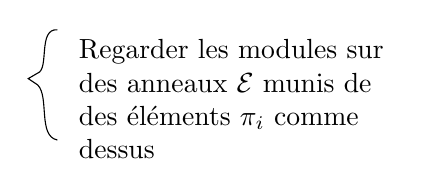
\begin{tikzpicture}[x=1cm,y=1cm]
\node[anchor=north west,align=left] at (.4,1.4) {Regarder les modules sur\\\deleted{des} anneaux $\mathcal E$ munis \deleted{\unsure{de}}\\des éléments $\pi_i$ comme\\dessus};
\draw (.25,1.4) .. controls (0,1.42) and (.15,.9) .. (0,.85) --(-.12,.78) --(0,.7) .. controls (.15,.55) and (0,.05) .. (.25,0);
\end{tikzpicture}}}

3. \deleted{Nous \unsure{voulons}} Partons enfin d'une \deleted{algèbre}\inserted{anneau} graduée $\mathcal E^*$ \deleted{sur $k$}, et posons nous la question de l'existence et \uline{l'unicité} d'une famille $(\pi_i)_{i\in\mathbb Z}$ d'éléments de $\mathcal E^*$, \inserted{satisfaisant $(1.1.)$} définissant la graduation, par $(1.3.)$ (donc par $(1.4)$). On \deleted{\unsure{supp}} suppose ici que
\mspage{3}
